\chapter{Introduction}
\label{sec:introduction}
This chapter will introduce the subject of mixed criticality embedded systems and the EU project "EMC\textsuperscript{2}" to the reader.

\section{Background}
%TODO: Better sources
Today, modern automotive systems contain a large number of Electronic Control Units (ECU)s, each controlling a subsystem of a specific criticality level such as safety-critical distance keeping system for platooning (see \ref{sec:platooning}) or non-critical entertainment systems \cite{website:emc2automotive}. Having the ECUs isolated ensures that the numerous critical and non-critical applications do not interfere with each other, thus it is a simple task to certify an individual ECU. However, this approach leads to an inefficient use of system resources and expensive system implementation \cite{burns2016}. In order to lower the cost of the collective system and increase system efficiency (utilization), applications of different criticality levels can be integrated into a single multicore platform, leading to a Mixed Criticality System (MCS). However, this approach increases system complexity, and hinders the certification of safety-critical systems \cite{zaki2016}. 
%TODO: wording
In order to facilitate the design, test, and certification of such systems, spatial and temporal partitioning can be used in the architecture of the system as described by \cite{zaki2016}.\\

Protecting the integrity of a component from the faults of another is desired in all systems hosting multiple applications. However, it is of higher significance if the different applications have different criticality levels. Without such protection all components on the same system would need to be engineered to the standards of the highest criticality level, potentially massively increasing development costs \cite{burns2016}.\\

%TODO: wording
The EU project "Embedded Multi-Core systems for Mixed Criticality applications in dynamic and changeable real-time environments" (EMC\textsuperscript{2}) was created in order to "find solutions for dynamic adaptability in open systems, provide handling of mixed criticality applications under real-time conditions, scalability and utmost flexibility, full scale deployment and management of integrated tool chains, through the entire lifecycle" \cite{website:emc2}. 

\subsection{Definition of safety-critical systems}
The term "safety-critical system" has many definitions, most quite similar. Most definitions relate to systems with the potential to harm humans if the system malfunctions. According to \cite{website:encyclopedia} it is defined as "A system in which any failure or design error has the potential to lead to loss of life." Further, \cite{website:dictionary} defines safety-critical systems as "A computer, electronic or electromechanical system whose failure may cause injury or death to human beings." A Wikipedia article, \cite{website:wikipedia}, defines a safety-critical system (or "life-critical system") as a system whose failure or malfunction may result in one (or more) of the following outcomes:
\begin{itemize}
\item death or serious injury to people
\item loss or severe damage to equipment/property
\item environmental harm
\end{itemize}
In this thesis, a safety-critical system will be defined as "a system whose failure may cause injury or death to human beings."

\subsection{Different levels of criticality}
Different names of levels of criticality are typically Safety Integrity Level (SIL), Automotive Safety Integrity Level (ASIL) and Development Assurance Level (DAL). The IEC 61508 standard \cite{IEC61508} defines four different levels and the ISO 26262 standard \cite{ISO26262} and the DO-178C standard \cite{DO178C} define five different levels each. These levels range from low to no hazard up to life-threatening or fatal in the event of a malfunction requiring the highest level of assurance that the dependent safety goals are sufficient and have been achieved.\\
%It should be noted that not all standards and papers on MCS assign to "criticality" the same meaning, an issue  explored by  Graydon and Bate [141], Esper et al. [123] and Paulitsch et al. [256]

In this report the number of criticality levels will be restricted to two: "safety-critical" and "non-critical". This is due to the constraints presented in section \ref{sec:mces} and \ref{sec:scope}.

\subsection{EMC\textsuperscript{2} Mixed criticality embedded system}
\label{sec:mces}
The current MCS is implemented on a Xilinx Zynq-7000. It employs two operating systems to handle applications of different criticality. A Linux General Purpose Operating System (GPOS) for non-safety critical applications and a Real-Time Operating System (RTOS) for safety-critical applications. 

%Hypervisor, FPGA, peripherals, virtualization

An overview of the system can be seen in Figure~\ref{fig:introduction_overview}.

\begin{figure}[H]
\centering
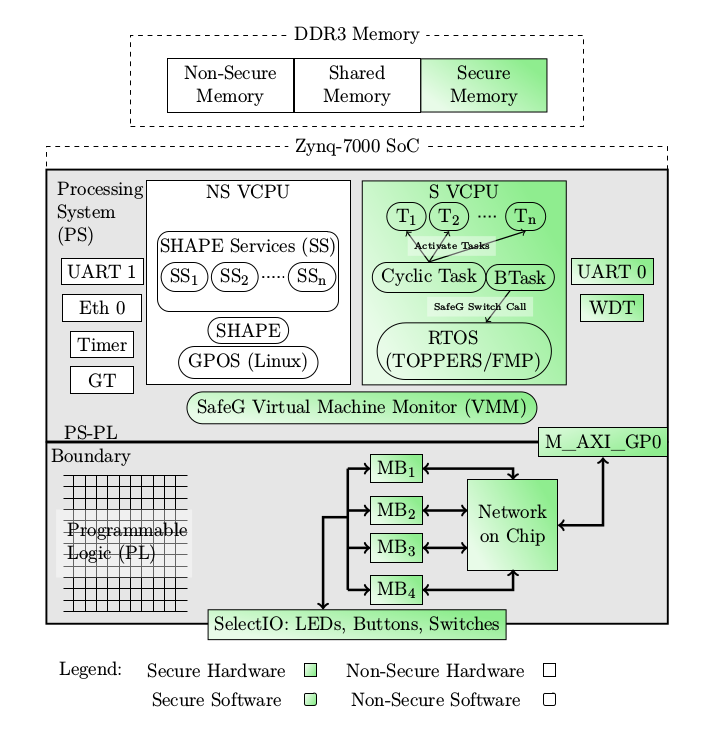
\includegraphics[width=\textwidth]{./img/introduction_overview.png}
\caption{System overview of the MCS in place.\cite{zaki2016}}\label{fig:introduction_overview}
\end{figure}

For more detailed information, see the report by \cite{zaki2016}.

\subsection{Platooning}
\label{sec:platooning}
%Wording
"The platooning concept can be defined as a collection of  vehicles that travel together, actively coordinated in formation. Some expected advantages of platooning include increased fuel and traffic  efficiency, safety and driver  comfort" \cite{bergenhem}.

\section{Problem statement}
\label{sec:problem}
%Implement safety-critical controller on the embedded system. 
A distance keeping control algorithm for platooning will be implemented on the embedded system described in \ref{sec:mces}. A demonstrator will be constructed in the form of a RC car capable of following a vehicle in front of it at a certain distance. It should be verified that no matter the computational load and eventual crashes of the Linux based non-critical system, the distance keeping algorithm on the RTOS never crashes.\\

This problem leads to the research question: 
\begin{itemize}
\item How well can a safety-critical control system perform when implemented on a mixed criticality system using virtualization?
\end{itemize}
alternatively:
\begin{itemize}
\item How, in a disciplined way, to reconcile the conflicting requirements of partitioning for safety assurance and sharing for efficient resource usage? \cite{burns2016}
\end{itemize}
alternatively:
\begin{itemize}
\item Is virtualization an efficient approach when trying to reconcile the conflicting requirements of partitioning for safety assurance and sharing for efficient resource usage when implementing a safety-critical control system?
\end{itemize}

\section{Purpose}
%TODO: Wording
Reducing the amount of computers in automotive systems would have many effects. Manufacturing costs would decrease and with fewer physical components maintenance costs would also decrease. However, the system complexity would increase and thereby increasing time and cost to design the system. To combat this the EMC\textsuperscript{2} project aims at creating platforms for easier development of MCS. %TODO: källa eller ändra wording

The EMC\textsuperscript{2} project lists several goals \cite{website:emc2goals}:
\begin{itemize}
\item Reduce the cost of the system design by 15\%
\item Reduce the effort and time required for re-validation and re-certification of systems after making changes by 15\%
\item Manage a complexity increase of 25\% with 10\% effort reduction
\item Achieve cross-sectorial reusability of Embedded Systems devices and architecture platforms that will be developed using the ARTEMIS JU results.
\end{itemize}

\section{Goals}
%TODO: Better wording?
In this project there are both team goals and individual goals that do not always necessarily align with each other. 

\subsection{Team goal}
The team consists of five master thesis students. The students areas of work are: control theory and system modeling, data aggregation, safety-critical communication in MCS, line following and system testing and finally safety-critical control in MCS. Together the team will build a vehicle capable of following a vehicle ahead of it while keeping inside road markers.

\subsection{Individual goal}
Verify quantitatively the performance of safety-critical distance keeping controller, see \ref{sec:research} Solve the problems described in \ref{sec:problem}.

\subsection{Scope}
\label{sec:scope}
%TODO: How much can the result be generalized?
The work of this thesis and the implementation on the demonstrator will build upon the work of \cite{zaki2016}.

The embedded computer is constrained to the Xilinx Zynq-7000 \footnote{\url{https://www.xilinx.com/products/silicon-devices/soc/zynq-7000.html}}. 

The thesis is produced at Alten AB. %TODO: Remove?

%Control algorithm will be designed by Daniel Roshanghias

%\section{Method}
\section{Research design}
\label{sec:research}
%TODO: verify source
The plan is to make an confirmatory investigation using qualitative data/operations. This is a mixed methods approach where the data is gathered using simulations of the environment \cite{creswell}. Gather data from simulations and from real tests, iterated many times.

%TODO: Kanske bättre i en annan del?
The position of the demonstrator will be read by a separate sensor of the same type as the one on the demonstrator. The performance of the control system and the embedded controller will be measured and compared with the same system without any non-critical computational load. This will also be done for a simulation of the system. The measures regarding control system performance will consist of 
\begin{itemize}
\item Response time
\item Overshoot
\item Settling time %Fel ord?
\end{itemize}
and the measures regarding embedded controller performance will consist of
\begin{itemize}
\item Missed deadlines
\item CPU utilization
\end{itemize}